\thispagestyle{cackithitoannone}
\pagestyle{cackithitoan}
\everymath{\color{cackithi}}
\graphicspath{{../cackithi/pic/}}
%\blfootnote{\color{cackithi}$^*$Khoa Toán Đại học Osnabrueck, CHLB Đức.}
\begingroup
\AddToShipoutPicture*{\put(0,616){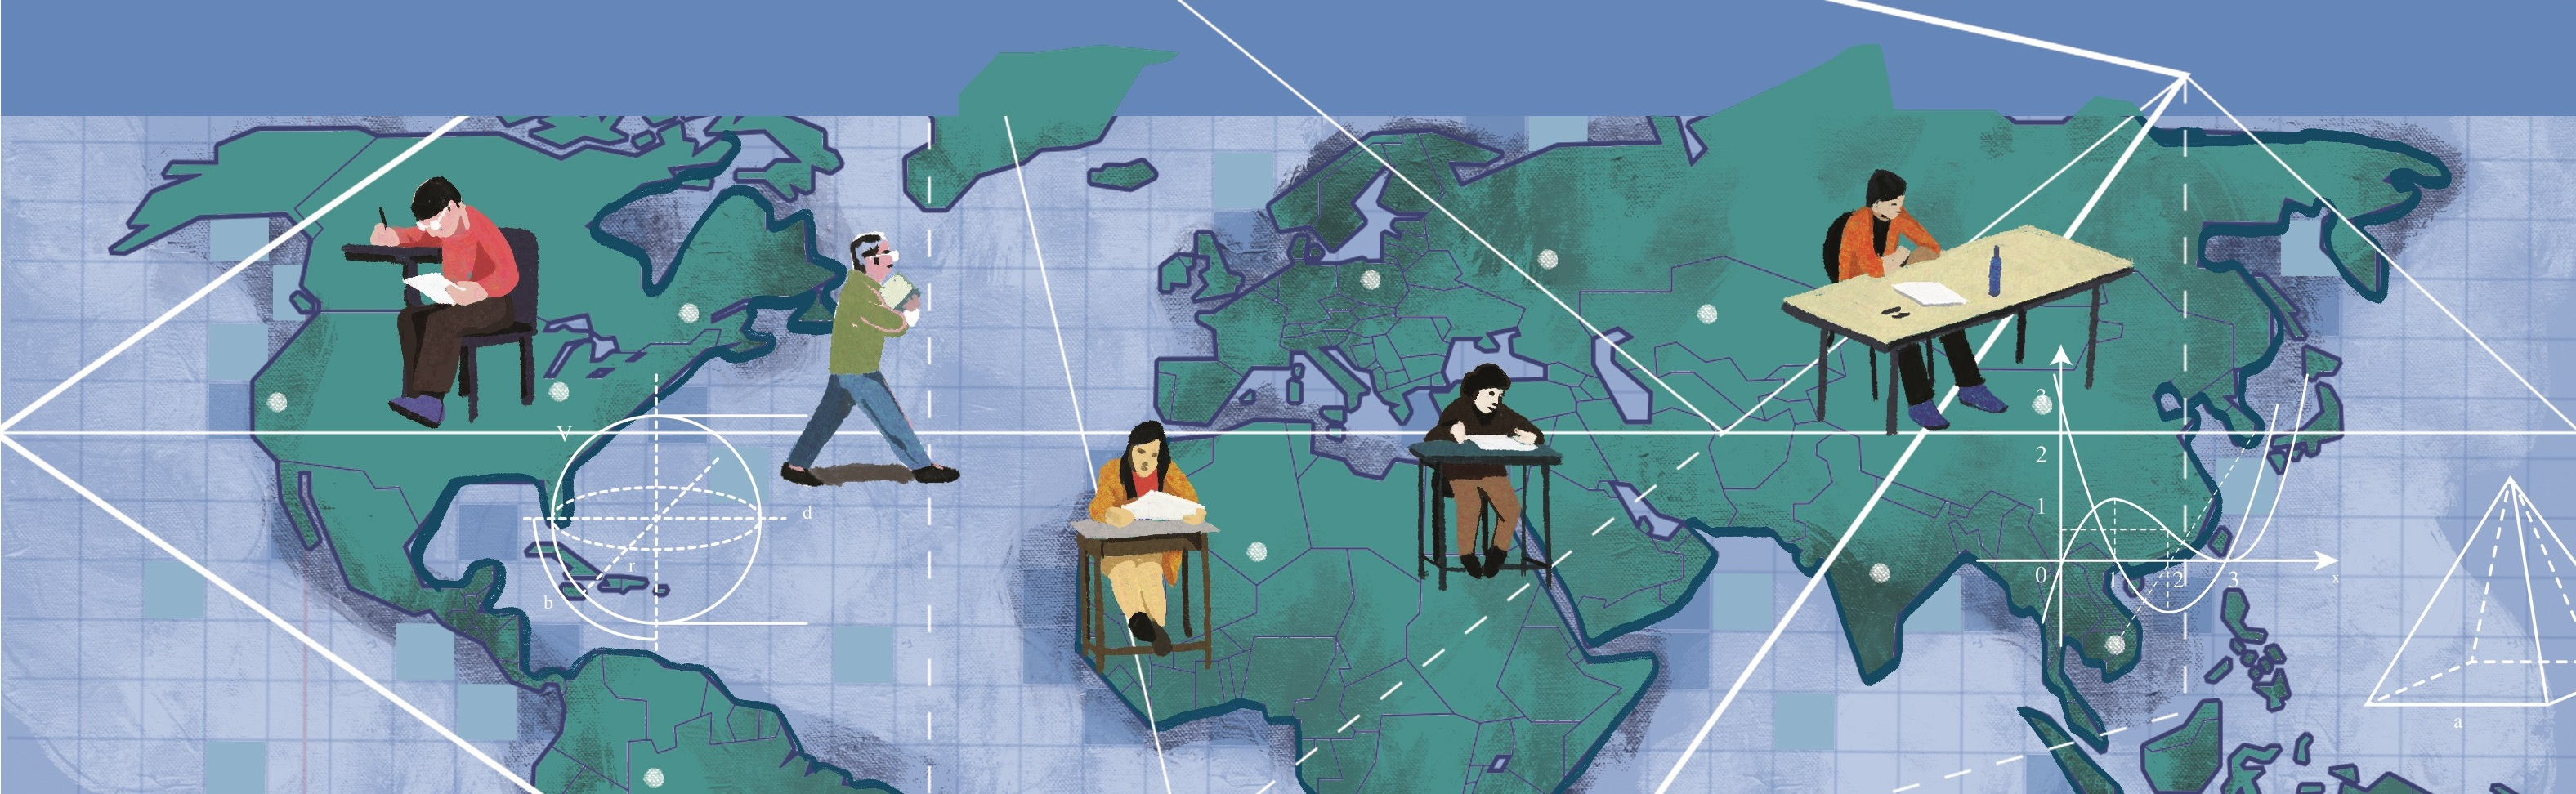
\includegraphics[width=19.3cm]{../bannercackithi}}}
\AddToShipoutPicture*{\put(145,575){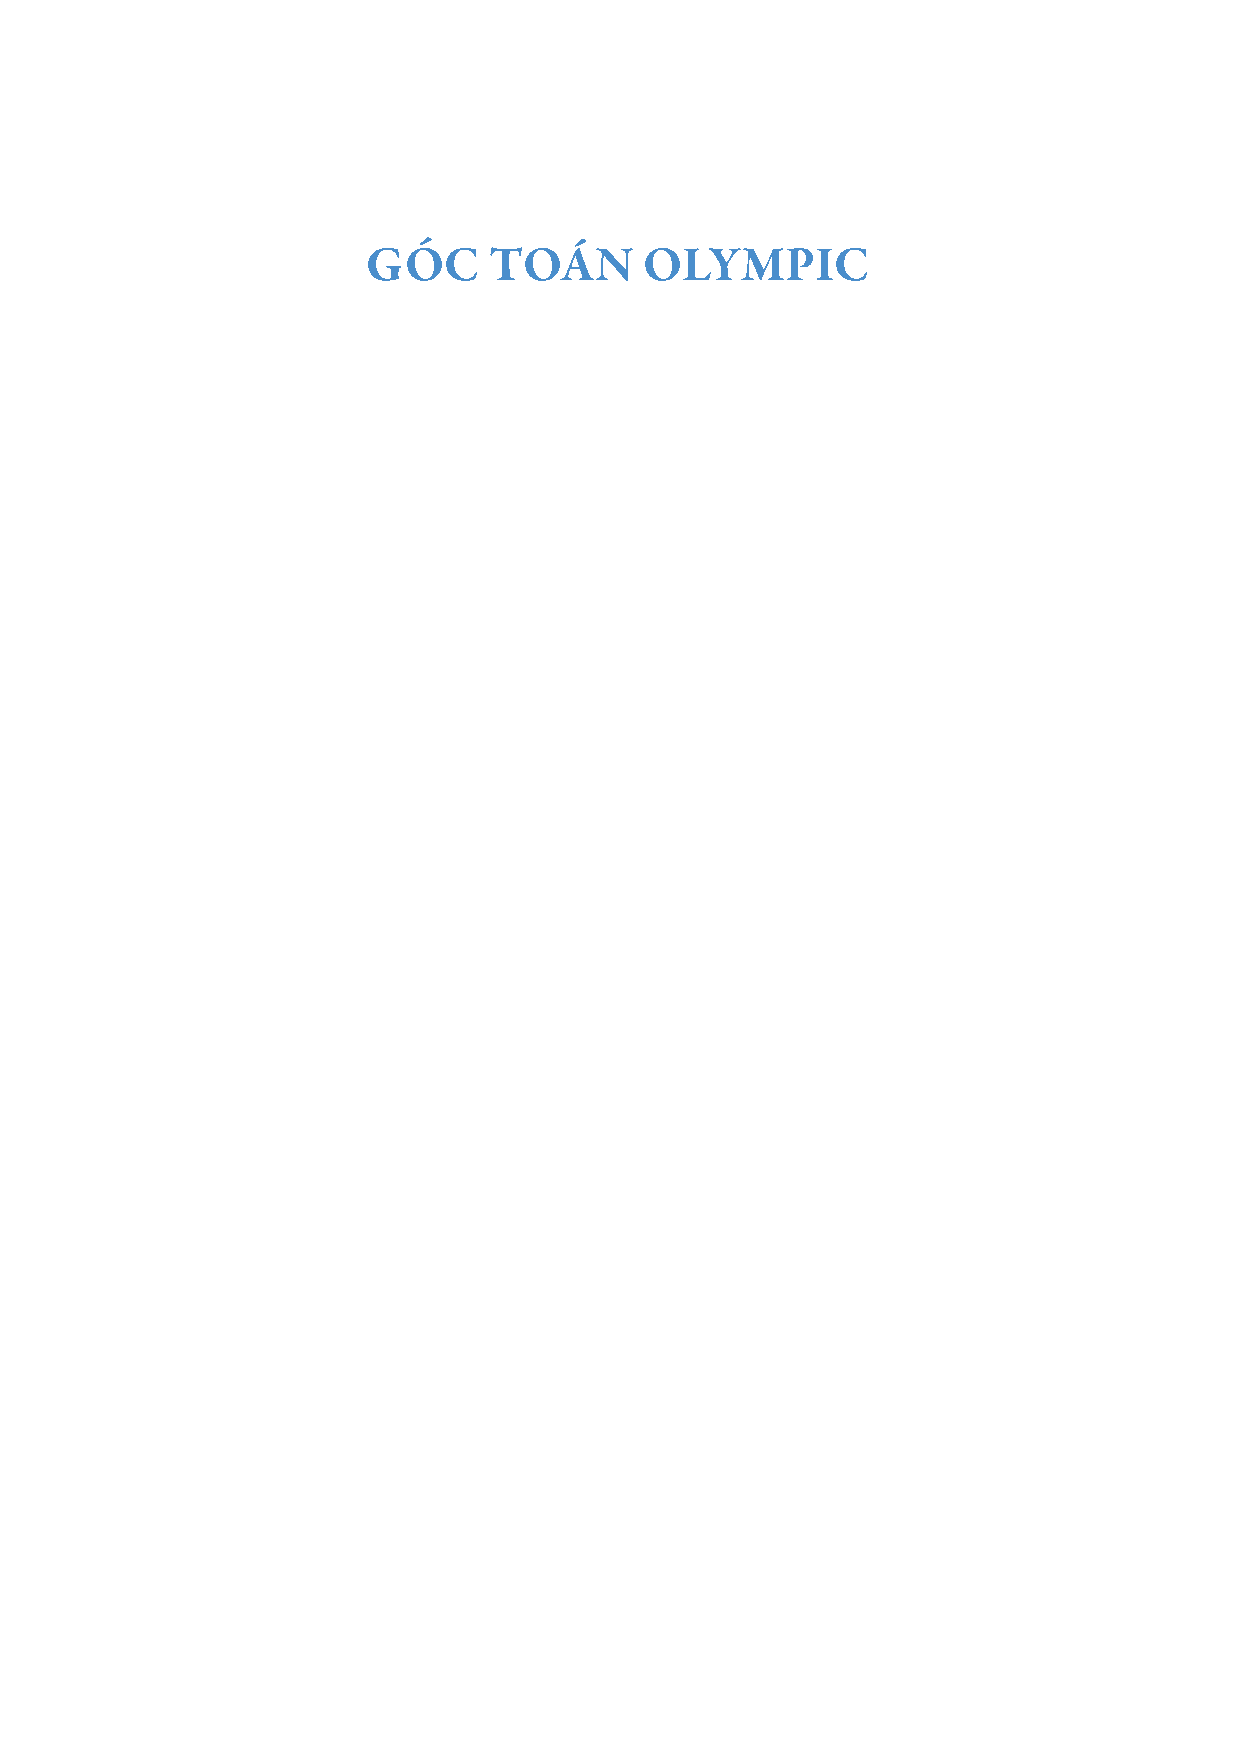
\includegraphics[scale=1]{../tieude1.pdf}}}
\centering
\endgroup
\vspace*{130pt}

\begin{multicols}{2}
	Trong phần đầu chuyên mục, chúng tôi sẽ trình bày với các bạn lời giải của các bài toán trong Kỳ thi toán Durer lần thứ XVI được tổ chức tại Hungary, đăng trong số báo $9/2023$. 
	\begin{figure}[H]
		\vspace*{-10pt}
		\centering
		\captionsetup{labelformat= empty, justification=centering}
		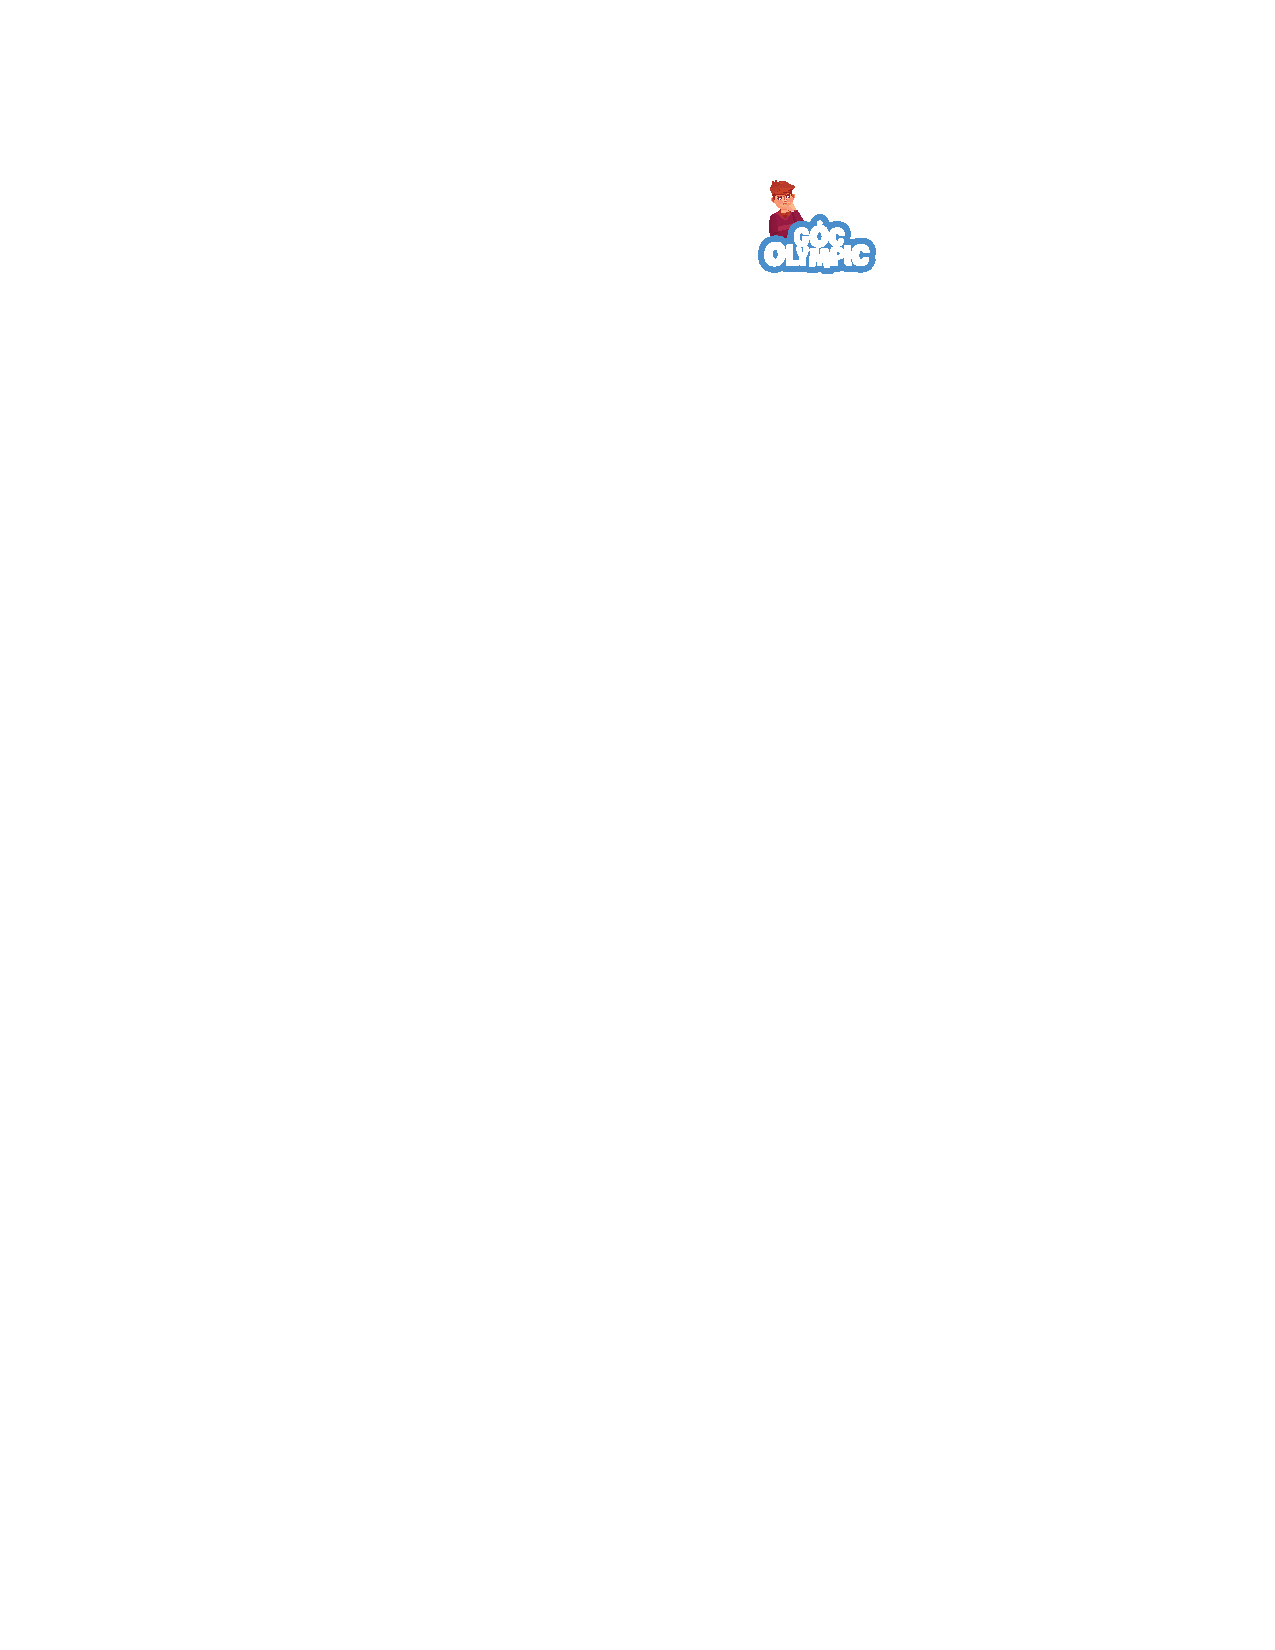
\includegraphics[width= 0.8\linewidth]{gocolympic}
%		\caption{\small\textit{\color{}}}
		\vspace*{-10pt}
	\end{figure}
	{\bf\color{cackithi} OC$\pmb{49}$.} Cho $ABC$ là tam giác cân. Cạnh đáy $BC$ dài $1$ cm, cạnh $AB$ và $AC$ dài $2$ cm. Gọi $F$ là trung điểm của $AB$ và $G$ là trung điểm của $AC.$ Gọi $(k)$ là đường tròn tiếp xúc với $AB$ và $AC$, tương ứng tại $F$ và $G$. Chứng minh rằng giao điểm của $CF$ và $BG$ thuộc đường tròn~$(k).$
	\vskip 0.1cm
	\textit{Lời giải.} 
	Gọi $I$ là giao điểm của $CF$ và $BG$ và $H$ là trung điểm của $BC.$ Như vậy $I$ là trọng tâm tam giác cân $ABC$ và $A, I, H$ thẳng hàng. Gọi $O$ là tâm của đường tròn $(k)$ thì do $AF, AG$ là tiếp tuyến với $(k)$ nên $O$ phải nằm trên đường phân giác của $\angle FAG.$ Như vậy $O$ nằm trên~$AH.$
	\vskip 0.1cm
	Do tam giác $BCG$ cân tại $C,$ ta đặt $\angle CGB=\angle CBG=\alpha.$ Vì $(k)$ tiếp xúc với $AC$ tại $G$ nên $OG\perp CG$ do đó $\angle OGI= 90^\circ -\alpha.$
	Mặt khác ta có
	\begin{align*}
		\angle OIG= \angle BIH= 90^\circ - \angle CBG=90^\circ- \alpha.
	\end{align*}
	Như vậy $\angle OGI=\angle OIG,$ ta suy ra $OG=OI,$ tức là $I$ nằm trên đường tròn $(k).$
	\begin{figure}[H]
		\vspace*{-10pt}
		\centering
		\captionsetup{labelformat= empty, justification=centering}
		\begin{tikzpicture}[cackithi,scale=0.85]
			\draw  (0.,0.)-- (4.,0.);
			\draw  (2.,7.75)-- (0.,0.);
			\draw  (2.,7.75)-- (4.,0.);
			\draw  (1.,3.875)-- (4.,0.);
			\draw  (3.,3.875)-- (0.,0.);
			\draw  (2.,7.75)-- (2.,0.);
			\draw  (2.,3.6162634408602155) circle (1.032930107526882cm);
			\draw  (2.,3.62)-- (3.,3.875);
			\draw [fill=white] (0.,0.) circle (2.0pt);
			\draw (-0.18,-0.5) node {$B$};
			\draw [fill=white] (4.,0.) circle (2.0pt);
			\draw (4.18,-0.5) node {$C$};
			\draw [fill=white] (2.,0.) circle (2.0pt);
			\draw (1.96,-0.5) node {$H$};
			\draw [fill=white] (2.,7.75) circle (2.0pt);
			\draw (2.14,8.11) node {$A$};
			\draw [fill=white] (1.,3.875) circle (2.0pt);
			\draw (0.74,4.07) node {$F$};
			\draw [fill=white] (3.,3.875) circle (2.0pt);
			\draw (3.34,4.1) node {$G$};
			\draw [fill=white] (2.,2.5833333333333335) circle (2.0pt);
			\draw (2.18,2.11) node {$I$};
			\draw [fill=white] (2.,3.62) circle (2.0pt);
			\draw (2.34,4.1) node {$O$};
		\end{tikzpicture}
		\vspace*{-10pt}
	\end{figure}
	{\bf\color{cackithi} OC$\pmb{50}$.} Khi Andris bước vào phòng, có các số $3$ và $24$ trên bảng. Trong một bước, nếu đã có các số (không nhất thiết phải khác nhau) $k$ và $n$ trên bảng, thì
	Andris có thể viết thêm số $kn + k + n$ lên bảng. 
	\vskip 0.1cm
	$(a)$ Liệu Andris có thể viết số  $9999999$ lên bảng sau một số bước?
	\vskip 0.1cm
	$(b)$ Cùng câu hỏi như phần $(a)$ cho số $99999999$?
	\vskip 0.1cm
	$(c)$ Cùng câu hỏi như phần $(a)$ cho số $48999999$?
	\vskip 0.1cm
	\textit{Lời giải.}
	Ta thấy cả hai số ban đầu trên bảng đều có dạng $n^2-1.$ Hơn nữa nếu hai số có dạng này thì số được viết thêm cũng có dạng này, thậy vậy
	\begin{align*}
		&(n^2-1)(m^2-1) + n^2-1 + m^2-1 \\
		= &(mn)^2-1.
	\end{align*} 
	$a)$ Vì  $9999999+1=10000000$ không phải số chính phương nên Andris không thể viết được số này.
	\vskip 0.1cm
	$b)$ Có thể viết được bằng các bước như sau:
	\vskip 0.1cm
	Trước tiên viết $3\times 24 + 3 + 24=99.$ Sau đó viết tiếp $99\times 99 + 99 + 99=9999.$ Và cuối cùng viết
	\begin{align*}
		9999\times 9999+ 9999+ 9999=99999999.
	\end{align*}
	$c)$ Nhận xét rằng với mọi số $k$ xuất hiện trên bảng thì $k+1$ chỉ có ước là $2$ hoặc $5$. Điều này đúng với hai số ban đầu là $3$ và $24$. Do $kn+k+n+1=(k+1)(n+1)$ nên khẳng định đúng với mọi số được viết thêm sau đó.
	\vskip 0.1cm
	Tuy nhiên do $48999999+1=49000000$ có ước là $7$ nên số $48999999$ không thể được viết lên bảng.
	\vskip 0.1cm
	{\bf\color{cackithi} OC$\pmb{51}$.} Có một trò chơi với một bảng ô vuông cỡ $3 \times 3$. Trong mỗi bước, người chơi lần lượt điền một trong các số $1$, $2$ hoặc $3$ vào một ô trống sao cho không có hai số giống nhau trong cùng một hàng hoặc trong cùng một cột. Nếu tất cả $9$ ô của bảng đều được điền số, người chơi đầu tiên thắng nhưng nếu trước đó có một thời điểm không thể điền số được nữa thì người chơi thứ hai thắng.
	\vskip 0.1cm
	Hỏi có cách nào để luôn chiến thắng nếu bạn được phép tùy chọn đi trước hoặc đi sau?
	\vskip 0.1cm
	\textit{Lời giải.} Ta sẽ chứng minh rằng người đi trước sẽ luôn có cách để chiến thắng.
	Nhận xét rằng nếu có một bộ $3$ ô, đôi một ở các hàng và cột phân biệt, đã được điền $3$ số phân biệt thì các ô còn trống đều có duy nhất một cách điền thỏa mãn đầu bài. Như vậy tất cả $9$ ô sẽ được điền và người chơi đi trước sẽ thắng. Một bộ ba như vậy được gọi là {\it bộ ba chiến thắng}. Ta sẽ chứng minh rằng người đi trước luôn có thể tạo ra một bộ ba chiến thắng.
	\begin{center}
		\begin{tikzpicture}[cackithi,scale=0.7]
			\draw (0,0) grid (3,3);
			\draw (1.5,0.5) node {$2$};
			\draw (2.5,1.5) node {$3$};
			\draw (0.5,2.5) node {$1$};
		\end{tikzpicture}
	\end{center}
	Trước tiên người đi trước điền số $1$ vào ô trung tâm của bảng. Nếu người đi sau điền số $2$ hoặc $3$ vào một ô ở góc thì ở lần đi tiếp theo người đi trước sẽ tạo ra được một bộ ba chiến thắng. Còn nếu người đi sau điền số $1$ vào một ô ở góc thì ở bước tiếp theo người đi trước sẽ tạo được một đường chéo gồm toàn số $1$. Tiếp theo dù người đi sau điền như thế nào thì người đi trước cũng tạo được một bộ ba chiến thắng. 
	\vskip 0.1cm
	Trường hợp người đi sau không điền vào ô ở góc thì người đi trước sau đó sẽ tạo được một hàng hoặc cột gồm $3$ số phân biệt. Ở bước tiếp theo dù người đi sau điền thế nào thì người đi trước cũng luôn tạo được một bộ ba chiến thắng. Như vậy người đi trước luôn thắng.  
	\vskip 0.1cm
	Trong phần cuối của chuyên mục kỳ này, chúng tôi sẽ giới thiệu với bạn đọc ba bài toán trong Kỳ thi Olympic Toán học Quốc gia Israel năm $2023$.
	\vskip 0.1cm
	{\bf\color{cackithi} OC$\pmb{58.}$} Có $2000$ người ngồi quanh một chiếc bàn tròn. Mỗi người trong số họ là người  thật thà (người luôn nói thật) hoặc kẻ  dối trá (người luôn nói dối). Biết rằng mỗi người đều nói: ``Ít nhất hai trong số ba người ngồi ngay sát bên phải của tôi là những kẻ dối trá". Hỏi có bao nhiêu người thật thà ngồi trong bàn?
	\vskip 0.1cm
	{\bf\color{cackithi} OC$\pmb{59}$.} Biết rằng các số nguyên không âm $x,y$ thỏa mãn
	\begin{align*}
		\sqrt{x}+\sqrt{x+60}=\sqrt{y}.
	\end{align*}
	Tìm giá trị lớn nhất có thể của $x$.
	\vskip 0.1cm
	{\bf\color{cackithi} OC$\pmb{60}$.} Liệu có tồn tại một tập hợp $S$ gồm $5783$ số thực phân biệt thỏa mãn điều kiện sau hay không:
	Với mọi $a,b\in S$ (không nhất thiết phải phân biệt) đều tồn tại hai số $c\neq d$ thuộc $S$ sao cho $a \times b=c+d$?
\end{multicols}